\documentclass{beamer}
\usepackage{listings}
\usepackage{xcolor}
\usepackage{graphicx}
\usepackage{float}
\usepackage{tikz}
\usetikzlibrary{decorations.pathmorphing, decorations.pathreplacing, decorations.shapes}
\usepackage{hyperref}
\usepackage{array}

\setbeamertemplate{navigation symbols}{}

\hypersetup{
	colorlinks=true,
	linkcolor=blue,
	filecolor=magenta,
	urlcolor=blue
}

\urlstyle{same}

\title{Bash Workshop II: Advanced}
\author{Frederick Yin}
\institute{JITech}
\date{2023}

\definecolor{codegreen}{rgb}{0,0.6,0}
\definecolor{codegray}{rgb}{0.5,0.5,0.5}
\definecolor{codepurple}{rgb}{0.58,0,0.82}
\definecolor{backcolour}{rgb}{0.95,0.95,0.92}

\lstdefinestyle{wksp}{
	backgroundcolor=\color{backcolour},
	commentstyle=\color{codegreen},
	keywordstyle=\color{magenta},
	numberstyle=\tiny\color{codegray},
	stringstyle=\color{codepurple},
	basicstyle=\ttfamily\footnotesize,
	breakatwhitespace=false,
	breaklines=true,
	captionpos=b,
	keepspaces=true,
	numbers=left,
	numbersep=5pt,
	showspaces=false,
	showstringspaces=false,
	showtabs=false,
	tabsize=4
}

\lstset{style=wksp}

\graphicspath{{./img/}}

\AtBeginSection[]{
	\begin{frame}
		\frametitle{Table of Contents}
		\tableofcontents[currentsection]
	\end{frame}
}

\renewcommand{\tt}{\texttt}

\begin{document}
\frame{\titlepage}

% !TeX root = bash.tex
\section{IV. Regex}
\begin{frame}
\frametitle{What's a regex}
\textbf{Regex}: ``regular expressions''
\newline \newline
It is a string… to search for strings.
\end{frame}

\begin{frame}[fragile]
\frametitle{What can (and can't) a regex do}
A regex can (or at least attempt to):
\begin{itemize}
    \item Match a cell phone number: \verb|[0-9]{11}|
    \item Match a .com domain: \verb|([A-Za-z0-9_\-]+\.)+com|
    \item Match \textit{Star Wars} subtitles but not \textit{Star Trek}:
        \verb!m | [tn]|b!\footnote{Credit: \url{https://xkcd.com/1313/}}
\end{itemize}
It cannnot:
\begin{itemize}
    \item Understand emotion (you want NLP)
    \item Generate AI art (you want stable diffusion)
    \item Moderate a Minecraft server (you want a real human)
\end{itemize}
\end{frame}

\begin{frame}
\frametitle{When to use regex?}
\begin{figure}[h]
    \centering
    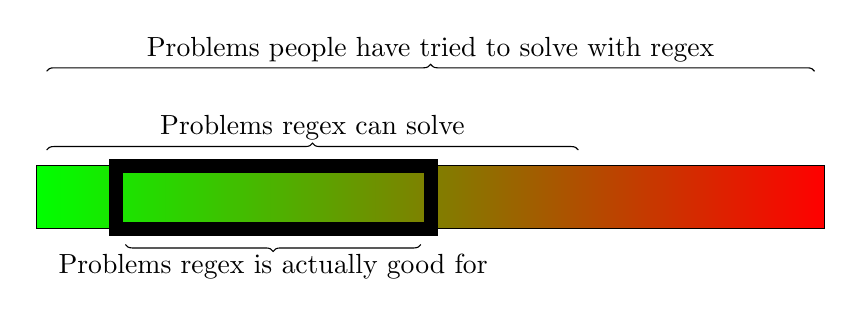
\begin{tikzpicture}
        \node (can-low)     at ( 0,  1)   {};
        \node (can-high)    at ( 7,  1)   {};
        \node (have-low)    at ( 0,  2)   {};
        \node (have-high)   at (10,  2)   {};
        \node (should-low)  at ( 1, -0.2) {};
        \node (should-high) at ( 5, -0.2) {};
        \draw[left color=green, right color=red] (0, 0) rectangle (10, 0.8);
        \draw[line width=5pt] (1, 0) rectangle (5, 0.8);
        \draw[decorate, decoration=brace] (can-low) -- (can-high)
            node[text centered, midway, above] {Problems regex can solve};
        \draw[decorate, decoration=brace] (have-low) -- (have-high)
            node[text centered, midway, above] {Problems people have tried to solve with regex};
        \draw[decorate, decoration={brace, mirror}] (should-low) -- (should-high)
            node[text centered, midway, below] {Problems regex is actually good for};
    \end{tikzpicture}
\end{figure}
\end{frame}

\begin{frame}
\frametitle{Regex is a mess}
\begin{block}{Quote}
I define UNIX as 30 definitions of regular expressions living under one roof.
\begin{flushright}
    — Donald Knuth\footnote{Digital Typography, ch. 33, p. 649 (1999)}
\end{flushright}
\end{block}

Two dominant standards:
\begin{itemize}
    \item \textbf{ERE} (Extended RegEx, POSIX compliant)
    \item \textbf{PCRE} (Perl Compatible RegEx, used in Perl and Python)
\end{itemize}
Our focus today will be ERE.
\end{frame}

\begin{frame}[fragile]
\frametitle{Common patterns (part 1)}
\begin{table}
    \centering
    \begin{tabular}{ll}
        \verb|.|            & any character \\
        \verb|\.|           & a literal dot \\
        \verb|[aeiou]|      & any vowel \\
        \verb|[^aeiou]|     & anything but a vowel \\
        \verb|[0-9]|        & any digit \\
        \verb|[A-Za-z]|     & any letter \\
        \verb|^|            & beginning of line \\
        \verb|$|            & end of line \\
        \verb|A?|           & zero or one A \\
        \verb|A+|           & one or more A's (\emph{Positive closure}) \\
        \verb|A*|           & zero or more A's (\emph{Kleene closure}) \\
        \verb|A{,6}|        & up to six A's \\
        \verb|A{4,6}|       & four to six A's \\
        \verb!(ls|cd|rm)!   & one of ls, cd, and rm
    \end{tabular}
\end{table}
\end{frame}

\begin{frame}[fragile]
\frametitle{Common patterns (part 2)}
\begin{table}
    \centering
    \begin{tabular}{ll}
        \verb|\w|           & \verb|[A-Za-z0-9_]| \\
        \verb|\W|           & anything that does not match \verb|\w| \\
        \verb|\s|           & whitespace (space, tab, linebreak, etc) \\
        \verb|\S|           & anything but whitespace \\
        \verb|\b|           & boundary of a word \\
        \verb|\B|           & you guessed it
    \end{tabular}
\end{table}
\end{frame}

\begin{frame}[fragile]
\frametitle{Quiz: Does it match?}
What strings does this regex match? \newline

\Large \verb!(^cat|cat$)! \normalsize

\begin{itemize}
    \item \verb|cat|                      % yes
    \item \verb|^cat$|                    % no
    \item \verb|cats|                     % yes
    \item \verb|cat /etc/fstab|           % yes
    \item \verb|I have a cat.|            % no
    \item \verb|Cats are the best.|       % no
    \item \verb|Concatenate these files|  % no
\end{itemize}
\end{frame}

\begin{frame}[fragile]
\frametitle{Quiz: Does it match?}
What matches \tt{+86 021-54749110} but not \tt{+86021-54749110}?
\begin{itemize}
    \item \verb|\+86\s+[0-9]{3}-[0-9]{8}|
    \item \verb|\+86\s*[0-9]{3}-[0-9]{8}| % this one
\end{itemize}

What does \Large \verb|[um]jicanvas.com| \normalsize match?
\begin{itemize}
    \item \tt{umjicanvas.com}
    \item \tt{jicanvas.com} % neither
\end{itemize}

\begin{block}{Challenge\footnote{Want more challenges? Try \url{https://alf.nu/RegexGolf}!}}
    How to fix this regex? \pause \verb|(um)?jicanvas\.com|
\end{block}
\end{frame}

\begin{frame}[fragile]
\frametitle{But how to use a regex, anyway?}
Try this in \tt{04-regex/}:
\begin{lstlisting}[language=bash]
$ grep -E '.+\..+@sjtu.edu.cn' faculty
\end{lstlisting}
\pause
\begin{block}{Observation}
    The regex matches all email addresses in the file \tt{faculty}
    that look like ``firstname.lastname@sjtu.edu.cn''.
\end{block}
\begin{block}{Challenge}
    Can you come up with something shorter?
\end{block}
\end{frame}

\begin{frame}[fragile]
\frametitle{One more example}
\begin{lstlisting}[language=bash]
$ grep -o -E '^[^@]{,8}' faculty
\end{lstlisting}
\pause
\begin{block}{Observation}
    This regex truncates each line after the 8th character or before @,
    whichever comes first.
\end{block}
\begin{block}{Explanation}
    \begin{tabular}{ll}
        \verb|^|    & From beginning of each line \\
        \verb|[^@]| & Match all characters except @ \\
        \verb|{,8}| & Until we reach max length 8
    \end{tabular}
\end{block}
\end{frame}

\begin{frame}[fragile]
\frametitle{Your turn}
Extract all course codes from \tt{04-regex/courses}. \newline

\begin{tabular}{lcl}
    VG100 Introduction to Engineering & & VG100 \\
    VM020 Machineshop Training & $\Longrightarrow$ & VM020 \\
    VP140 Physics I & & VP140 \\
    VP141 Physics Lab I & & VP141
\end{tabular}
\pause
\begin{block}{Solution (one version)}
\begin{lstlisting}[language=bash]
$ grep -oE 'V[A-Z][0-9]+' courses
\end{lstlisting}
\end{block}
\end{frame}

\begin{frame}[fragile]
\frametitle{Find and replace with \tt{sed}}
\tt{sed} is a powerful tool for transforming text.
We will be using one very specific syntax:
\begin{lstlisting}[language=bash]
$ COMMAND | sed 's/FIND/REPLACE/'
\end{lstlisting}
Use \tt{-E} for regex. This command redacts all the IPv4 addresses in the
file \tt{ipv4}:
\begin{lstlisting}[language=bash]
$ sed -E 's/([0-9]{1,3}\.){3}[0-9]{1,3}/redacted/g' \
    ipv4
\end{lstlisting}
\begin{block}{Note}
    Without the \tt{g} at the end, \tt{sed} will skip to the
    next line after only one replacement.
\end{block}
\end{frame}

\begin{frame}[fragile]
\frametitle{Groups in regex}
What if you only want to redact the subnet (i.e. last part) of the IP addresses?
\textbf{Capturing groups} will be useful.
\begin{lstlisting}[language=bash]
$ sed -E 's/(([0-9]{1,3}\.){3})[0-9]{1,3}/\1xxx/g' \
    ipv4
\end{lstlisting}
\end{frame}

% !TeX root = bash.tex
\section{V. Bash Scripting}
\begin{frame}[fragile]
\frametitle{Bash is a programming language}
Let's say you want to print many files at once.

Try this one-liner:
\begin{lstlisting}[language=bash]
$ for i in {01..05}; do \
    cat um-logo-$i.txt; \
done
\end{lstlisting}
\end{frame}

\begin{frame}[fragile]
\frametitle{Variables}
A variable in bash is defined this way:
\begin{lstlisting}[language=bash]
$ i=0
$ s='s'
\end{lstlisting}
Surprisingly these do \textbf{not} work:
\begin{lstlisting}[language=bash]
$ i = 0
$ s = 's'
\end{lstlisting}
Use them with a dollar sign:
\begin{lstlisting}[language=bash]
$ echo $i  # 0
\end{lstlisting}
\end{frame}

\begin{frame}[fragile]
\frametitle{Environment variables}
Let's say you're downloading something from a completely legal website, and you
want the traffic to go through your local proxy server for completely legal reasons.
You need to set an \textbf{environment variable}:
\begin{lstlisting}[language=bash]
# your local proxy
$ export HTTPS_PROXY=http://localhost:8080/
# download the thing
$ curl https://legal.website/legal-thing/
\end{lstlisting}
This does the same thing, but subsequent commands do not have access to it:
\begin{lstlisting}[language=bash]
$ HTTPS_PROXY=http://localhost:8080/ \
    curl https://legal.website/legal-thing/
\end{lstlisting}
\end{frame}

\begin{frame}[fragile]
\frametitle{Note about long commands}
In this section, commands can be rather long. You may type them in a command line,
or you can edit a shell script (\tt{something.sh}) and run it
(\tt{bash ./something.sh}).
\begin{table}
    \begin{tabular}{m{12em} cc}
        \hline
        & Type in CLI & Run a script file \\
        \hline
        \verb|\| at the end of line & Necessary & Unnecessary \\
        \verb|;| between two commands on the same line & Necessary & Necessary \\
        \hline
    \end{tabular}
\end{table}
\end{frame}

\begin{frame}
\frametitle{Exit status}
When a program exits, it emits an \textbf{exit status} (also called exit code).
By convention, an exit status of 0 implies success, and everything else means
something went wrong (consult respective man pages).

\begin{block}{Note}
    When you \tt{return 0;} at the end of \tt{int main()}, you are
    emitting an exit status of zero.
\end{block}
\end{frame}

\begin{frame}[fragile]
\frametitle{\textbf{if} statements}
\begin{lstlisting}[language=bash]
if COMMAND; then
    # CODE
elif COMMAND2; then
    # CODE2
else
    # CODE3
fi
\end{lstlisting}
where \tt{COMMAND} can be
\begin{itemize}
    \item A CLI command; \tt{CODE} will run if exit status is zero
    \item \tt{[[ CONDITION ]]} where you compare strings with \tt{==}
        or numbers with \tt{-eq}
\end{itemize}
\begin{block}{Note}
    This is way too much to unpack here, but you can check out
    \url{https://www.gnu.org/software/bash/manual/html_node/Conditional-Constructs.html#index-_005b_005b}
\end{block}
\end{frame}

\begin{frame}[fragile]
\frametitle{\textbf{for} statements}
\begin{lstlisting}[language=bash]
for VARIABLE in LIST; do
    # CODE
    # use VARIABLE with $VARIABLE
done
\end{lstlisting}
where \tt{LIST} is commonly a range, e.g. \verb|{01..10}|, or the output of
another command, e.g. \verb|$(ls)|.
\begin{block}{Note}
    In bash, a string can be split into a list with respect to whitespace.
    Therefore, \verb|$(ls)| only works as expected if no path contains whitespace.
\end{block}
\end{frame}


\begin{frame}
\frametitle{The End}
\vspace{1cm}
\centering \Huge {Thank You For Coming!}
\end{frame}

\begin{frame}
\frametitle{Credits}
\begin{itemize}
    \item Monkey User, Regex Explained.
        \url{https://www.monkeyuser.com/2020/regex-explained/}
\end{itemize}
\end{frame}
\end{document}
